\documentclass[11pt]{article}


%\documentclass[11 pt]{article}
\usepackage{graphicx}
\usepackage{float}



\usepackage[utf8]{inputenc}

\usepackage[square,sort,comma,numbers]{natbib}
\bibliographystyle{abbrvnat}
\setcitestyle{authoryear,open={(},close={)}} %Citation-related commands

\usepackage{setspace}

\usepackage{pdflscape}
\doublespacing
\usepackage[dvipsnames]{xcolor}
\usepackage{lineno}
\linenumbers
\usepackage{multicol}
\usepackage{hyperref}
\hypersetup{
	colorlinks=false,
%	linkcolor=blue,
%	filecolor=magenta,      
%	urlcolor=cyan,
	pdftitle={Overleaf Example},
	pdfpagemode=FullScreen,
}

\addtolength{\oddsidemargin}{-2.5cm}
\addtolength{\evensidemargin}{-1.5cm}

\addtolength{\textwidth}{5.5cm}

\addtolength{\topmargin}{-.875in}
\addtolength{\textheight}{1.75in}

%\author{Pending}


\begin{document}
%\title{Understanding the emergence of viral variants of concern via Bayesian molecular clock model selection}
\begin{flushright}

%\today
\end{flushright}
\begin{center}
	\begin{LARGE}
	\textbf{The phylodynamic threshold of measurably evolving populations}
	\end{LARGE}

Ariane Weber$^{1,*}$, Sanni Översti$^{1}$, Julia Kende$^{2}$, and Sebastian Duchene$^{3,4,*}$.
\end{center}

$^{1}$ Pending.

$^{2}$ Institut Pasteur, Université Paris Cité, Bioinformatics and Biostatistics Hub, Paris, France.

$^{3}$ ED-ID unit, Dept of Computational Biology, Institut Pasteur, Paris, France.

$^{4}$ Peter Doherty Institute for Infection and Immunity, Dept of Microbiology and Immunology, University of Melbourne, Melbourne, Australia.


*email: weber@gea.mpg.de, sduchene@pasteur.fr
%		\maketitle

\begin{Large}
	\textbf{Abstract}
\end{Large}

Pending.

\textbf{Keywords:} Measurably evolving populations, phylodynamic threshold, molecular clock, Bayesian phylogenetics, microbial evolution.

%\begin{Large}
%\textbf{Significance statement}
%\end{Large}

%Genome data from the ongoing SARS-CoV-2 pandemic have been key to detect and trace the emergence of variants of concern, with increase transmissibility and impacts on vaccine efficacy. At a genetic level, variants have much higher numbers of defining mutations than is expected under the standard mutation rate of the virus. We analysed genome data of the four variants of concern recognised by the WHO to uncover their evolutionary dynamics. We find that the lineages of the virus that preceded these variants had a mutation rate at least 4 times faster than the baseline, a process that was sustained over a few months, but which does not appear permanent.
%Up to 120 words. 

\section{Introduction}
Molecular sequence data have become nearly ubiquitous for studying the evolution of modern and ancient organisms. A fundamental concept in molecular evolution is the `molecular clock', which posits that substitutions accumulate roughly constantly over time \citep{zuckerkandl1965evolutionary}. An underlying assumption of the classic molecular clock is that selective constraints are negligible for most sites and over time. The development of molecular clock models as a statistical processes relax this and other assumptions by allowing for rate variation among branches in phylogenetic trees (reviewed by \cite{ho2014molecular}).

Molecular clock models necessarily involve two key quantities, the evolutionary timescale and the `evolutionary rate', with the latter representing the combination of mutations and substitutions that accrue over time. However, evolutionary times and rates cannot be jointly identified using genetic sequence data alone, that is they are undentifiable (\cite{dos2013unbearable} and reviewed by \cite{bromham2018bayesian}). To overcome this problem, all molecular clock methods require prior assumption about evolutionary times or rates, known as a `molecular clock calibration'. For example, one can constraint the age of the common ancestor between two lineages (i.e. an internal node in a phylogenetic tree) to a given time or fix the evolutionary rate to a known value. The choice of calibration depends on the information available and its reliability \citep{warnock2012exploring, duchene2014impact}. 

\subsection{Measurably evolving populations}
Rapidly evolving organisms, notably viruses and some bacteria, have been found to accrue an appreciable number of mutations over the sampling timescale. Influenza viruses, for example, have evolutionary rates of around $6\times10^{-3}$ subs/site/year \citep{ghafari2021purifying, sanjuan2012molecular}. Assuming a genome size of 13,500 Kb, one would expect to observe one mutation every 4 to 5 days ($\frac{365\ days/year}{13500\ sites\ \times\ 6\times10^{-3}subs/site/year}\approx4.5\ days/subs$). If genome samples are collected over the course of a few weeks, then the sampling times themselves can be used to calibrate the molecular clock, a practice known as `tip calibration' (reviewed by \cite{rieux2016inferences}). Data sets for which the molecular clock can be calibrated using sequence sampling times are considered to have been sampled from a `measurably evolving population' \citep{drummond2003measurably}.

Advances in sequencing technologies have dramatically expanded the range of organisms from which data sets can be considered to have been sampled from a measurably evolving population. First, ancient DNA techniques have effectively expanded the genome sampling window for many organisms \citep{spyrou2019ancient, duchene2020recovery}. One of many examples, is mitochrondrial DNA recovered from dogs from 36,000 years before present \citep{thalmann2013complete}, which was found to be sufficient to calibrate its molecular clock. Second, whole genome sequencing has meant that data sets of `slowly' evolving microbes often carry sufficient information for calibrating the molecular clock \citep{biek2015measurably}. The causative agent of tuberculosis, the bacterium \textit{Mycobacterium tuberculosis}, was commonly considered to evolve too slowly for calibrating the molecular clock using samples collected over a few years \cite{duchene2016genome}. However, data sets involving the full genome, of about 4.4 Mb, have demonstrated that a genome sampling window of a few decades might be sufficient for reliable clock calibration \citep{menardo2019molecular}.

\subsection{The phylodynamic threshold}
The emergence of SARS-CoV-2 saw the rapid generation of genome data from the early stages of the outbreak, with phylodynamic analyses conducted in near to real-time \citep{attwood2022phylogenetic}. The first attempts to estimate the evolutionary rate and time of origin were highly uncertain due to two factors; a narrow sampling window and low genetic diversity. In \cite{duchene2020temporal} Bayesian phylodynamic analyses of the available genomes were conducted as the outbreak unfolded, such that the number of genomes and the width of the sampling window increased over time and ranged from 22 genomes sampled over 31 days to 122 genomes sampled over 63 days. The early estimates of the evolutionary rate and time of origin had high uncertainty, but they rapidly converged to values that were robust to the addition of more data. The term `phylodynamic threshold' refers to the time where an organism has accrued a sufficient amount of genetic change \textit{since its emergence} for tip-calibrations to be informative \citep{duchene2020temporal}.  

The terms \textit{phylodynamic threshold} and \textit{measurably evolving population} are different, albeit related, concepts. A population is measurably evolving if the samples available are sufficiently informative as to warrant tip calibration. In contrast, the phylodynamic threshold is the amount of time over which we would need to draw samples for the data set to behave as a measurably evolving population. For a recently evolving pathogen it would simply correspond to the point in time at which it has accrued sufficient genetic diversity since its emergence, under the condition that the data have been collected constantly over time. In contrast, an ancient organism may have attained its phylodynamic threshold, with substantial genetic diversity, but drawing a samples from a very short time window may fail to capture a representative amount of such genetic diversity (fig. \ref{figure:Fig1}).

\subsection{Temporal signal}
Tests of temporal signal are designed to assess our ability to extract information from data for estimating evolutionary rates and timescales (reviewed by \cite{rieux2016inferences}). These tests do not differentiate between recently emerging organisms (i.e. they have not attained their phylodynamic threshold; fig. \ref{figure:Fig1}a) and those with narrow sampling windows (i.e. the data cannot be treated as being drawn from a measurably evolving population; fig. \ref{figure:Fig1}d), both of which may lack temporal signal. Additionally, these tests assume that the phylogenetic model adequately captures the evolutionary process. However, pervasive evolutionary rate variation (an 'overdispersed molecular clock') may lead to rejection of temporal signal under a strict clock model. Thus, temporal signal is not solely a property of the data but also depends on model performance. Recent research suggests that the choice of tree prior and molecular clock model significantly impacts the sensitivity and specificity of temporal signal tests, with relaxed molecular clocks being particularly effective \citep{tay2024assessing}.

Various methods exist for assessing temporal signal, including root-to-tip regression \citep{buonagurio1986evolution, gojobori1990molecular, drummond2003inference}, date-randomization tests \citep{ramsden2009hantavirus, duchene2015performance, duchene2018inferring, trovao2015host}, and the Bayesian Evaluation of Temporal Signal (BETS; \cite{duchene2020bayesian}). Root-to-tip regression fits a regression of root-to-tip distance against sampling time, with the $R^2$ value indicating clocklike behavior. Date-randomization tests compare evolutionary rate estimates using correct sampling times against permutations. BETS evaluates whether including sampling times improves model performance using Bayes factors. Importantly, a lack of temporal signal does not necessarily preclude estimating evolutionary rates and timescales, as additional sources of information (e.g., prior rate estimates or known internal node ages) can provide valid calibration, albeit potentially less precise than sequence sampling times for microbial pathogens.

A lack of temporal signal is typically considered to be associated with unreliable molecular clock estimates. In practice, this situation is thought to be alleviated by broadening the sampling window or by including more ancient samples. However, the presence and direction of a possible bias in estimates of evolutionary rates and timescales is poorly understood. 


%Tests of temporal signal were devised to determine our ability to draw information from the data to estimate evolutionary rates and timescales. Fundamentally, these tests do not make the distinction between organisms that are recently emerging (i.e. they have not attained their phylodynamic threshold; fig \ref{figure:Fig1}a) or those for which the sampling window is too narrow (i.e. the data cannot be treated as being drawn from a measurably evolving population; Fig \ref{figure:Fig1}d). 

%Moreover, tests of temporal signal make the assumption that evolutionary process is reasonably well captured by the phylogenetic model. If evolutionary rate variation is pervasive, known as an `overdispersed molecular clock' then a testing for temporal signal under a strict molecular clock model may reject temporal signal. Thus, temporal signal is not an inherent property of the data, but a combination of the information in the data and the performance of the model. In fact, recent research has suggested that the choice of the tree prior and molecular clock model can considerably impact the sensitivity and specificity of tests of temporal signal, with the relaxed molecular clock being particularly effective \citep{tay2024assessing}.

%The simplest method to assess temporal signal is the root-to-tip regression \citep{buonagurio1986evolution, gojobori1990molecular, drummond2003inference}, which consists of fitting a regression of the distance from the root to the tips as a function of the sampling time. The coefficient of determination, $R^2$, measures the degree of clocklike behaviour, and the regression parameters, slope and x-intercept correspond to estimates of the evolutionary rate and age of the root node, respectively. This method is very popular, with a range of user-friendly implementations \citep{rambaut2016exploring, featherstone2024clockor2}. However, the data points in the root to tip regression are not statistically independent, and therefore p-values are generally not reported. For this reason this method is used as a visual inspection, rather than a formal statistical test of temporal signal.

%Other tests of temporal signal test the association between sampling times and genetic divergence. The date-randomisation test \citep{ramsden2009hantavirus} consists of comparing the estimate of the evolutionary rate with the correct sampling times and with multiple permutations of the sampling times. The analysis of the data is considered to have temporal signal if the estimate with the correct sampling times does not overlap with the permutations. This test is available in Bayesian and maximum likelihood frameworks, and thus it benefits from a a range of molecular clock models \citep{duchene2015performance, duchene2018inferring, trovao2015host}.

%The Bayesian Evaluation of Temporal Signal, BETS, is an approach that is grounded on formal model testing \citep{duchene2020bayesian}. The premise of this test is whether the inclusion of sampling times in a Bayesian phylogenetic model improves results in better performance than their exclusion, where model performance is typically quantified using Bayes factors. Like the date-randomisation tests, BETS can exploit the full range of Bayesian phylogenetic models.

%Critically, a lack of temporal signal under any of the approaches above means that sampling times are not informative under the model in question, but this situation does not necessarily preclude a researcher from fitting a molecular clock and estimating evolutionary rates and timescales. Additional sources of information, such as prior evolutionary rate estimates for closely related organisms or known ages of internal nodes (and fossils where available) are entirely valid sources of calibration \citep{zhang2016total}, although they might be less precise than sequence sampling times, especially for microbial pathogens.

\begin{landscape}
	\begin{figure}[H]
		\begin{center}
			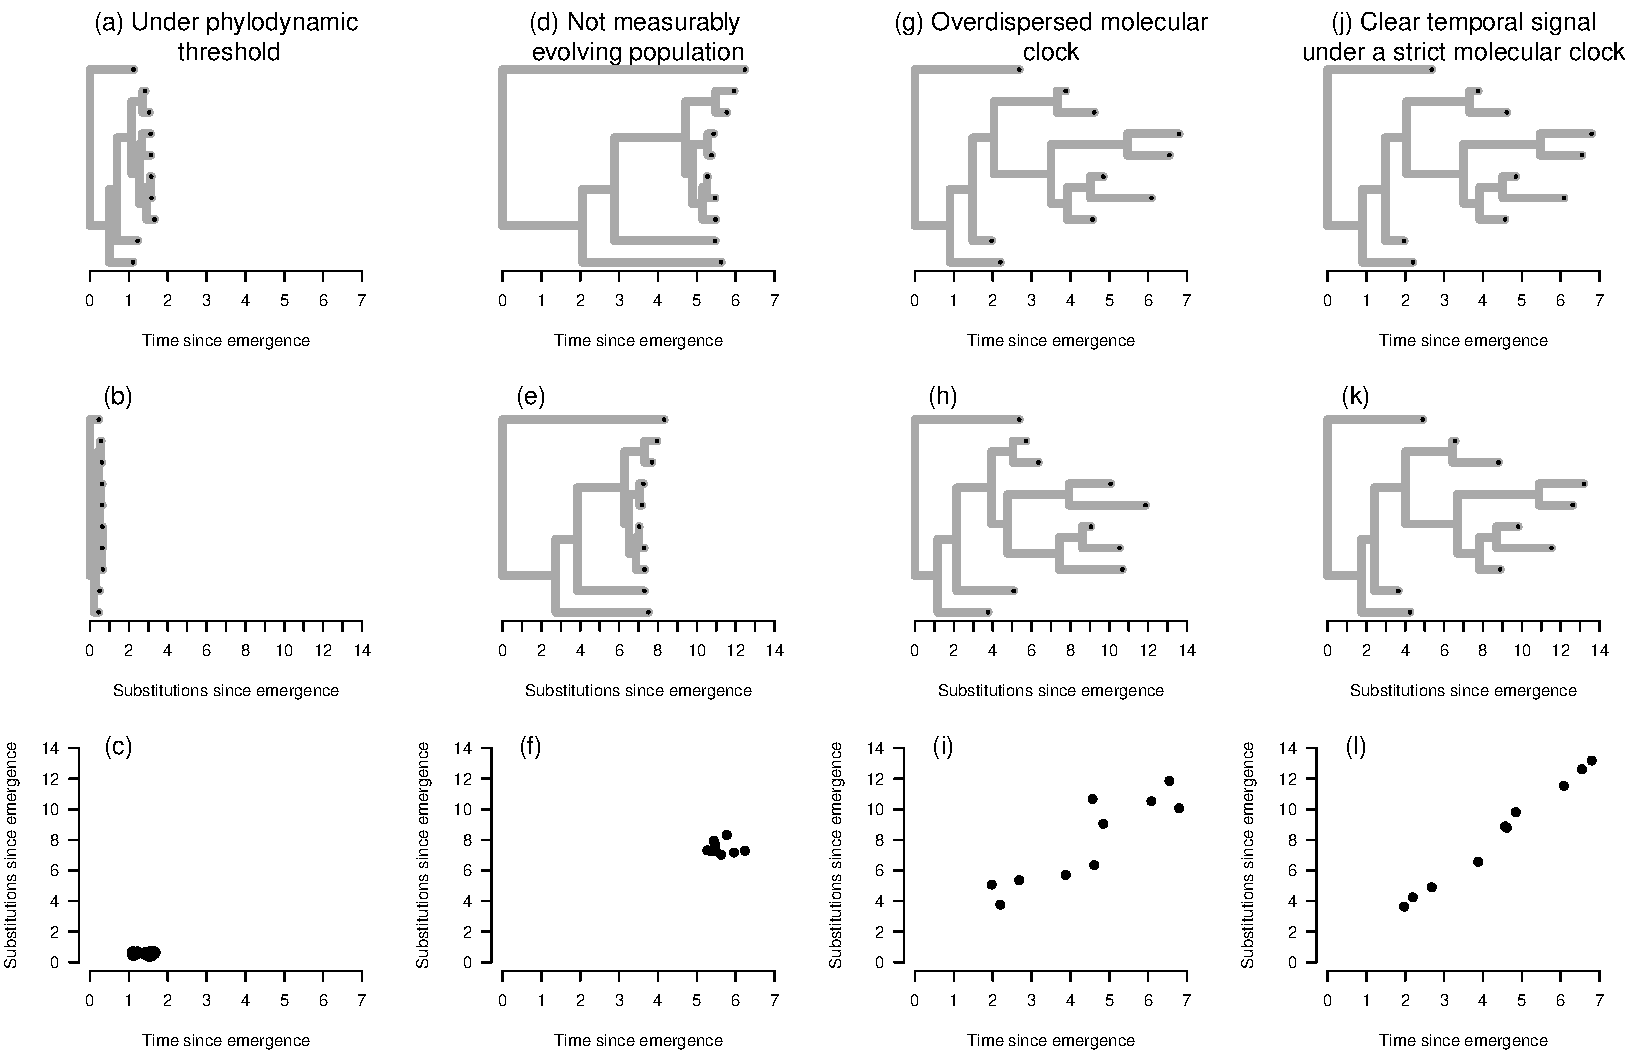
\includegraphics[scale=0.7, angle=0]{examples_temp_signal_thresholds_meps.pdf}
			\caption{Examples of situations where temporal signal is typically not detected. An organism that has not attained its phylodynamic threshold has a recent time of emergence (with a phylogenetic time tree shown in (a)) because it has not had sufficient time to accrue an appreciable number of substitutions (phylogenetic tree with branch lengths in subs/site, i.e. a `phylogram', shown in (b)), such that it is not possible to establish a statistical relationship between molecular evolution (substitutions) and time (shown in (c)). Sequence data from an organism that has evolved for a substantial amount of time may have been sampled over a very narrow window of time that is not sufficient to treat it as a measurably evolving population (time tree in (d) and phylogram in (e)), which results in no temporal signal (root-to-tip regression in (f)). A data set may involve a wide sampling window of time and from a population that has attained its phylodynamic threshold, but an overdispersed molecular clock (substantial rate variation among lineages; panels (g) - (i)) may result in a lack of temporal signal. In (j) through (l) we show the situation where an organism has attained its phylodynamic threshold and it has been sampled for sufficiently long, as to produce a clear relationship between molecular evolution and time, and unequivocal temporal signal.}
			\label{figure:Fig1}
		\end{center}
		%		\centering
	\end{figure}
\end{landscape}


\section{Results}
In this study we sought to pinpoint the impact of sampling strategies on these estimates. We focused our attention on two major problems for emerging microbes and studies involving ancient DNA. First, we varied the sampling window of a population that has attained its phylodynamic threshold. Second, we subsampled a population over time to vary the number of ancient samples, leading to a temporal sampling bias. Finally, we illustrate these results in an empirical data set of Hepatitis B virus (HBV) that includes a large number of ancient samples \citep{kocher2021ten}. This virus has been the subject of intense research due to its close association with human populations and complex evolutionary dynamics \citep{paraskevis2013dating, ross2018paradox, kahila2012tracing}.

\subsection{Sampling windows relative to the phylodynamic threshold}
We simulated sequence data that resembled the evolution of HBV, a double-stranded DNA (dsDNA) virus that has evolved in humans for around 10 thousand years \citep{kocher2021ten}. Our synthetic data had a genome length of 3,200 Kb and an evolutionary rate of $1.5\time10^{-5}$ subs/site/year \citep{kocher2021ten, muhlemann2018ancient}. Under these conditions we expect to observe one mutation every 20 years ($\frac{1}{3200\ sites \times\ 1.5\times10^{-5}subs/site/year}\approx20\ years$). This number is important for the design of our simulation experiments: 20 years is the time we would expect for it to attain its phylodynamic threshold and it is would typically be the required sampling window to detect temporal signal.

\subsection{Calibration windows for tips}
We conceived a simulation process under which the evolutionary timescale had an expected time of 10 thousand years and with a sampling window of 0, 10, 20, 200 , or 2,000 years. A sampling window spanning 0 years results in ultrametric trees with the sampling times providing no calibration information. In contrast, a sampling window of 10 years is half of the phylodynamic threshold and is expected to have weak temporal signal (see fig. \ref{figure:Fig1}(d)-(f)). Sampling windows of 20 years (the phylodynamic threshold) or wider are expected to behave as measurably evolving populations and with increasingly strong temporal signal (see fig. \ref{figure:Fig1}(j)-(l)). All our simulations were analysed under Bayesian phylogenetic framework, as implemented in the BEASTv2.5 platform \citep{bouckaert2019beast}.

All our simulations produced posterior estimated that included the correct value used to generate the data (i.e. high coverage). Increasingly wide sampling windows improved the precision of the estimates, while still including the correct value. We do not observe a systematic bias associated with the sampling window width, contrary to the expectation that low temporal signal necessarily results in an underestimation of the evolutionary rate and an overestimation of the tree height \citep{duchene2015performance}.

This result is largely expected due to our configuration of the prior. Notably, the prior on the phylogenetic tree and the evolutionary rate are particularly influential for estimating evolutionary rates and timescales (for a detailed investigation see \cite{tay2024assessing}).Here tree prior is a constant-size coalescent for which the prior on the population size (known as $\Theta$) is an exponential distribution with mean of 5,000, which matches the value used to generate the data. Similarly, the evolutionary rate had a prior in the form of a $\Gamma$ distribution with shape=1.5 and rate=$10^{6}$, whose mean is shape$\times$rate$=1.5\times10^{-6}$ and thus also matches the `true' value. Although these priors are centred on the correct values, they are vague, and it is important to note than in all cases, the posterior distribution of the evolutionary rate and tree height was narrower than the prior, meaning that even in the absence of sampling times the sequence data provide some information about these two parameters.


\textcolor{purple}{Note to self: That precision generally improves, but there does not seem to be a systematic bias if the prior is reasonable. When the prior is unreasonable, then we do need to sample quite past the phylodynamic threshold}



\textcolor{red}{WRITING UP TO HERE. THE REST IS RUBBISH!}




\begin{landscape}
	\begin{figure}[H]
		\begin{center}
			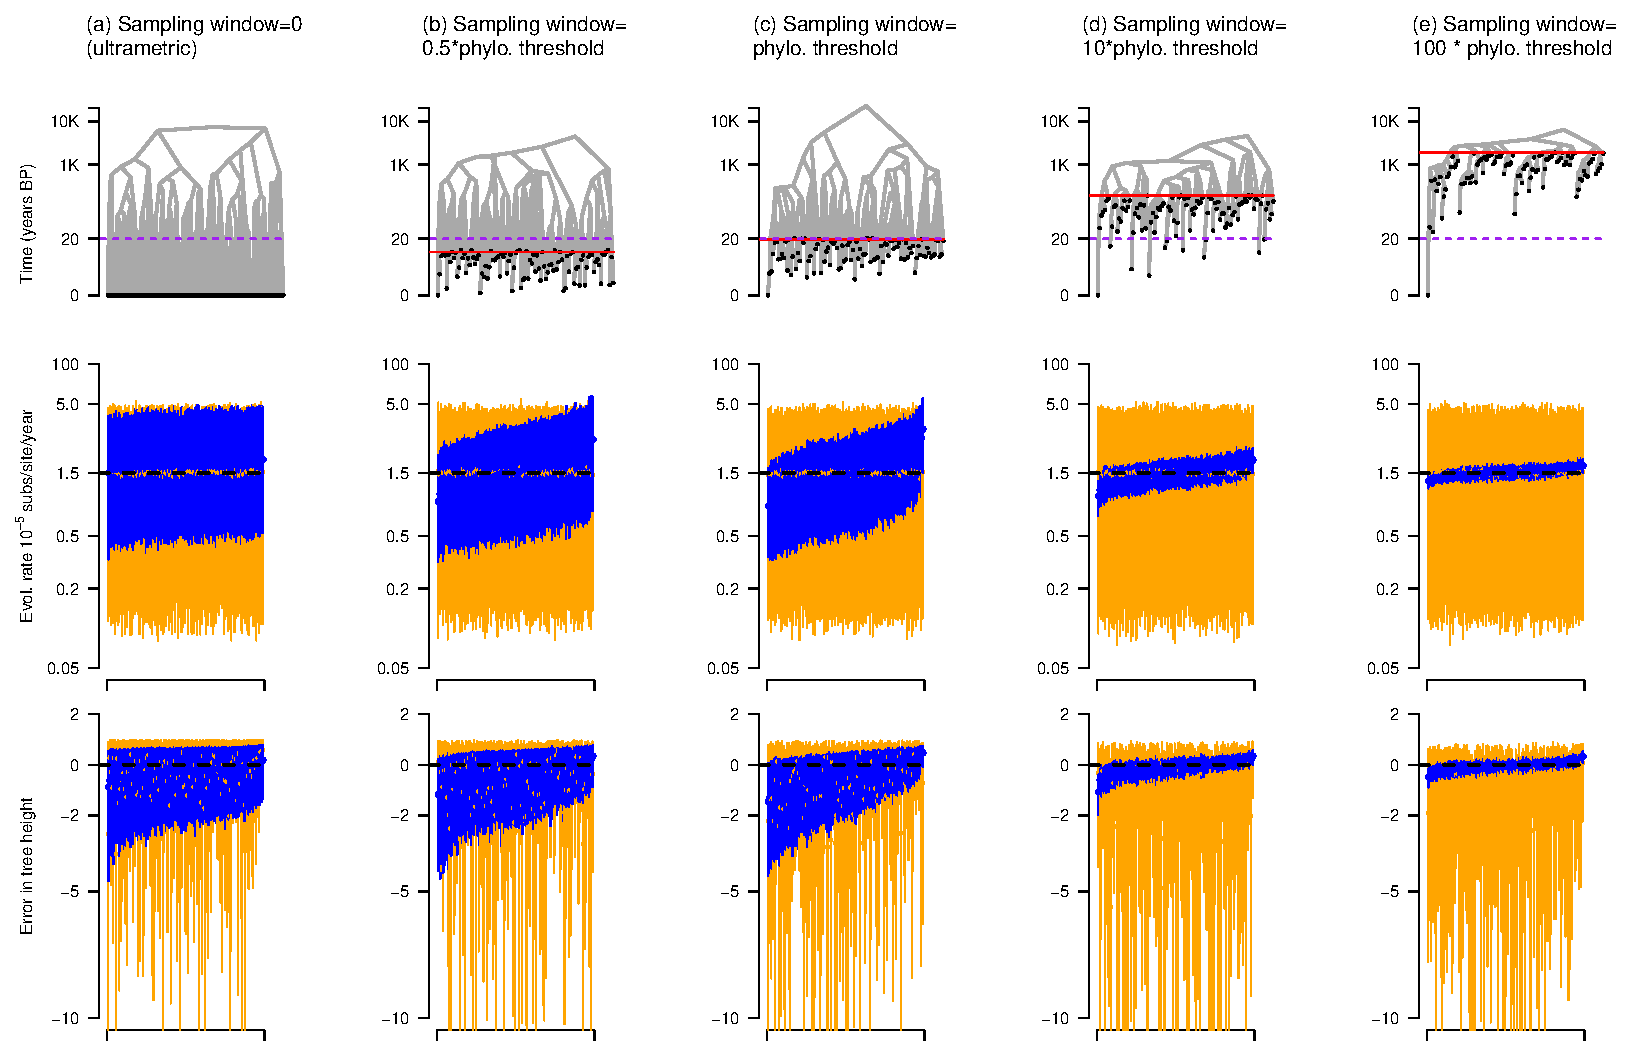
\includegraphics[scale=0.7, angle=0]{summary_all_estimates_correct_prior.pdf}
			\caption{Simulations of varying sampling window widths. Each column corresponds to a simulation setting: (a) is for ultrametric trees where all samples are collected at the same point in time, (b) is for the situation where the sampling window is 10 years (half the phylodynamic threshold), (c) is where the sampling window is exactly the phylodynamic threshold of 20 years. Scenarios (d) and (e) denote sampling windows that are 10 and 100 times the phylodynamic threshold. The first row is an example of a simulated phylogenetic tree with branch lengths scaled in units of time. The black circles represent genomic samples. The purple dashed line is is the phylodynamic threshold and the solid red line is for the oldest sample, such that it represents the sampling window. Note that time here is shown in log$_{10}$ scale. The second row is the estimated evolutionary rate over 100 simulations. The dashed black line is the value used to generate the data (i.e. the ground truth), the blue bars are the posterior, and those in orange are the prior. For the prior and the posterior we use solid circles to show the mean estimate. The third row is the estimate of the error in tree height (the age of the tree). The error in tree height is calculated as the $\frac{true-estimated}{true}$.}
			\label{figure:Fig2}
		\end{center}
		%		\centering
	\end{figure}
\end{landscape}

\begin{landscape}
	\begin{figure}[H]
		\begin{center}
			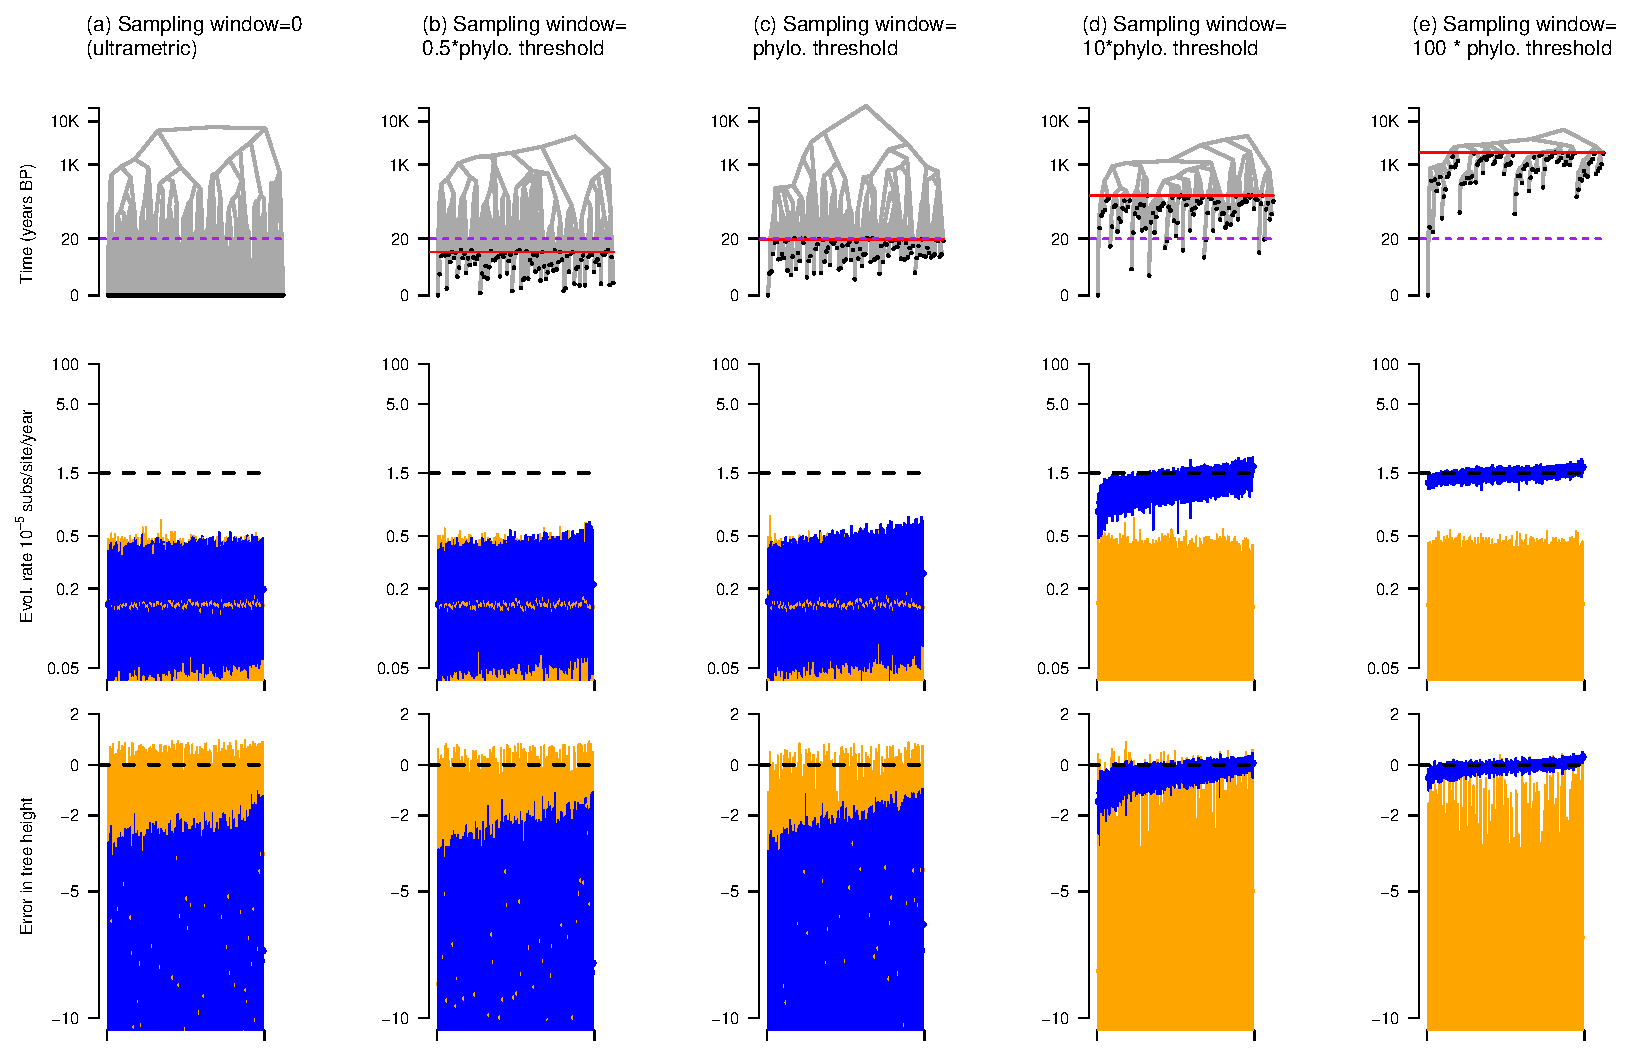
\includegraphics[scale=0.7, angle=0]{summary_all_estimates_misleading_prior.pdf}
			\caption{Simulations of varying sampling window widths. The colours, labels and legends match those from fig \ref{figure:Fig2}. However, in these analyses we deliberate use misleading priors on two key parameters, with a exponential distribution with mean 5,000 for the coalescent population size (true value=5,000), and a $\Gamma(shape=1.5, rate=10^{6})$ with mean=$1.5\times10^{-6}$ (true value=$1.5\times10^{-5}$).}
			\label{figure:Fig3}
		\end{center}
		%		\centering
	\end{figure}
\end{landscape}


%\begin{landscape}
\begin{figure}[H]
	\begin{center}
		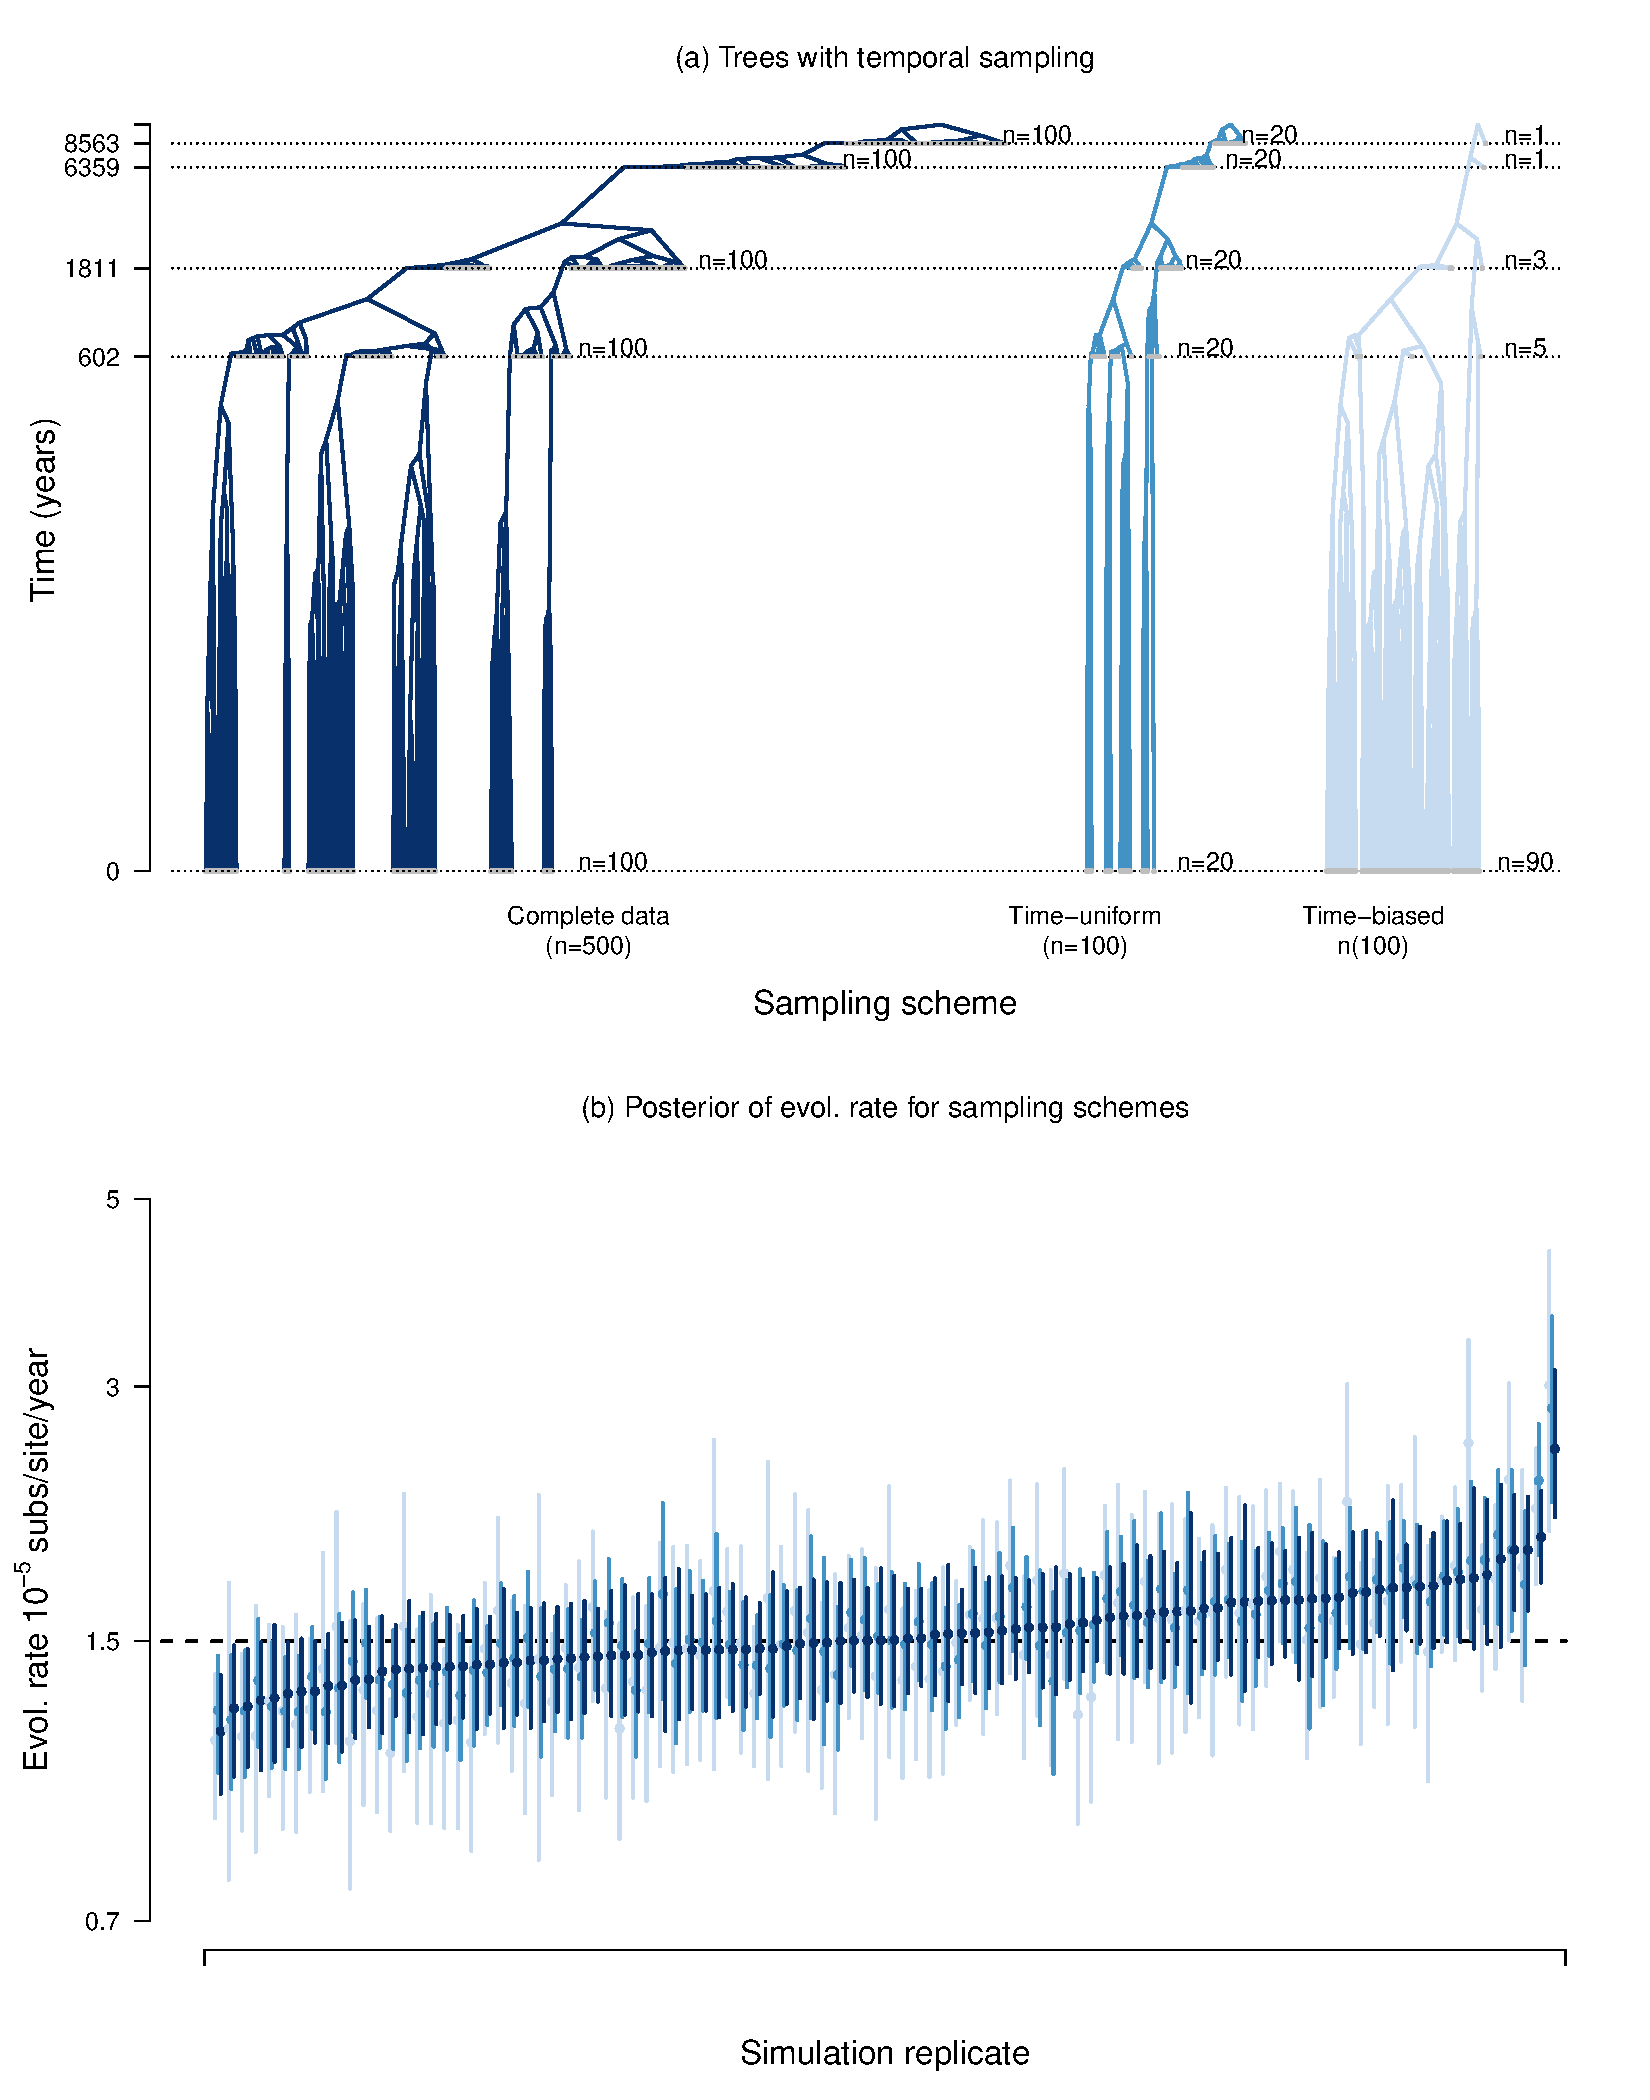
\includegraphics[scale=0.6, angle=0]{sampling_bias_summary_trees_rates.pdf}
		\caption{Trees plot thing pending}
		\label{figure:Fig4}
	\end{center}
		%		\centering
\end{figure}
%\end{landscape}


\begin{figure}[H]
	\begin{center}
		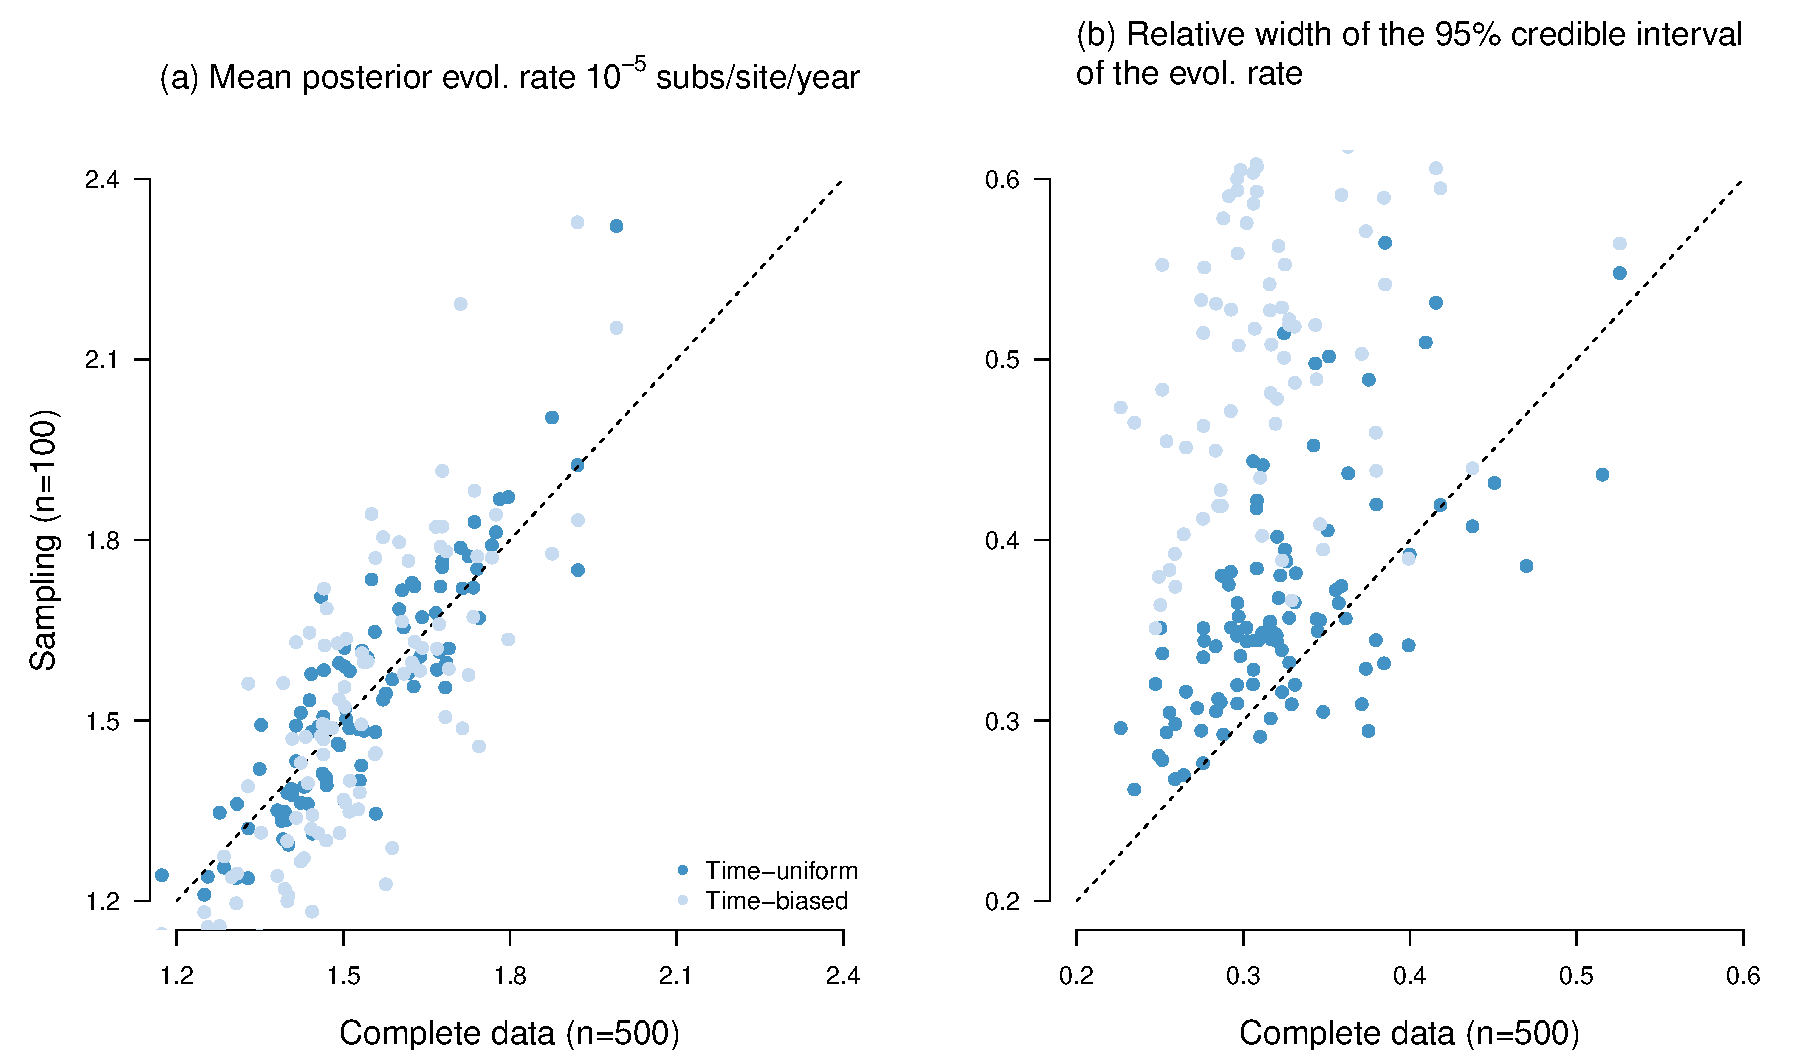
\includegraphics[scale=0.4, angle=0]{sampling_bias_summary_rates.pdf}
		\caption{Trees plot thing pending}
		\label{figure:Fig5}
	\end{center}
	%		\centering
\end{figure}

	

\begin{table}[H]
	\begin{center}
		\caption{placeholder for any tables}
		\label{table:table2}
		\begin{tabular}{c|c|c|c|c|c|c}
			\textbf{Model} & \textbf{ps logML} & \textbf{ss logML} & \textbf{ps rank} & \textbf{ss rank} & \textbf{ps BF} & \textbf{ss BF} \\ 
			\hline
		FLC shared stems & -55427.65 & -55428.17 & 1 & 1 & 0 & 0 \\ 
		FLC stems & -55431.50 & -55432.14 & 2 & 2 & -3.85 & -3.97 \\
		UCG	&	-55433.64 & -55434.26 & 3 & 3 & -6.00 & -6.01 \\
		UCLN & -55434.32 & -55434.69 & 4 & 4 & -6.67 & -6.52 \\ 
		FLC shared clades+stems & -55443.30 & -55443.50 & 5 & 5 & -15.64 & -15.34 \\ 
		SC & -55443.53 & -55444.21 & 6 & 6 & -15.88 & -16.04\\ 
		FLC shared clades & -55449.89 & -55450.52 & 7 & 7 & -22.23 & -22.35 \\ 
		FLC clades+stems & -55453.91 & -55454.58 & 8 & 8 & -26.25 & -26.41 \\ 
%		UCED & -55455.28 & -55455.04 & 9 & 9 & -27.63 & -26.87 \\ This one is too weird. Exclude?
		FLC & -55461.87 & -55462.54 & 9 & 9 & -34.21 & -34.38 \\ 
		\end{tabular}
	\end{center}
\end{table}





\section{Discussion}
Pending.
\section{Materials and methods}
Pending.


\section{Acknowledgements}
This work was supported by the Australian Research Council (DE190100805) and the Medical Research Future Fund (MRF9200006). This research was undertaken using the LIEF HPC-GPGPU Facility hosted at the University of Melbourne. This Facility was established with the assistance of LIEF Grant LE170100200. We acknowledge efforts by originating and submitting laboratories for the sequence data in GISAID EpiCoV on which our analyses are based. We are also grateful to Prof. Edward Holmes for useful suggestions and comments on ideas developed in this study.



%\bibliographystyle{plain}
\bibliography{References}

\end{document}